%%%%%%%%%%%%%%%%%%%%%%%%%%%%%%%%%%%%%%%%%%%%%%%%%%%%%%%%%%%%%%%%%%%%%%%%%%%%%%
%% AMS-LaTeX Paper
%%%%%%%%%%%%%%%%%%%%%%%%%%%%%%%%%%%%%%%%%%%%%%%%%%%%%%%%%%%%%%%%%%%%%%%%%%%%%%
\documentclass[12pt,leqno]{amsart}
\pdfoutput=1
\usepackage{amsmath, amssymb, amsthm}
% \usepackage{rsfso}
\usepackage[svgnames]{xcolor}
\usepackage{tikz}
\usetikzlibrary{arrows,cd}
\tikzset{>=latex}
\usepackage{mathtools}
%\usepackage[alwaysadjust]{paralist}
\usepackage[alphabetic]{amsrefs}
\usepackage[T1]{fontenc}
\usepackage{mathptmx}
\usepackage{microtype}
\linespread{1.06}
\usepackage[colorlinks = true,
  linkcolor  = DarkBlue,
  urlcolor   = DarkRed,
  citecolor  = DarkGreen]{hyperref}
\hypersetup{
  pdftitle={The simplicial complexes package for Macaulay2},
  pdfauthor={Ben Hersey, Gregory G. Smith, and Alexandre Zotine}
}
%% --Extras------------------------------------------------------------------
\usepackage{caption}
\usepackage{subcaption}
%% --LAYOUT-------------------------------------------------------------------
\usepackage[centering, includeheadfoot, hmargin=1.0in, tmargin=1.0in,
  bmargin=1in, headheight=6pt]{geometry}
%% --DISPLAY CODE------------------------------------------------------------
\usepackage{listings}
\lstset{
  basicstyle=\ttfamily,
  mathescape
}
\usepackage{stix}
%% --OTHER ENVIRONMENTS-------------------------------------------------------
\newtheorem{lemma}{Lemma}[section]
\newtheorem{theorem}[lemma]{Theorem}
\newtheorem{maintheorem}{Theorem}
\newtheorem{corollary}[lemma]{Corollary}
\newtheorem{proposition}[lemma]{Proposition}
\theoremstyle{definition}
\newtheorem{definition}[lemma]{Definition}
\newtheorem{remark}[lemma]{Remark}
\newtheorem{example}[lemma]{Example}
% \newenvironment{example}
% {\pushQED{\qed}\renewcommand{\qedsymbol}{$\diamond$}\examplex}
% {\popQED\endexamplex}
\newtheorem{question}[lemma]{Question}
\renewcommand{\theequation}{\arabic{section}.\arabic{lemma}.\arabic{equation}}
\renewcommand{\thetable}{\arabic{section}.\arabic{lemma}.\arabic{equation}}
\renewcommand{\thesubsection}{\arabic{section}}

%% --MATH---------------------------------------------------------------------
\newcommand{\PP}{\ensuremath{\mathbb{P}}}
%% Operators
\DeclareMathOperator{\Hom}{Hom}
\DeclareMathOperator{\Proj}{Proj}
\DeclareMathOperator{\Spec}{Spec}
\DeclareUnicodeCharacter{0393}{\Gamma}
\DeclareUnicodeCharacter{0394}{\Delta}
\DeclareUnicodeCharacter{22C8}{\bowtie}
\DeclareUnicodeCharacter{29D3}{\fbowtie}
%\DeclareUnicodeCharacter{}


%%%%%%%%%%%%%%%%%%%%%%%%%%%%%%%%%%%%%%%%%%%%%%%%%%%%%%%%%%%%%%%%%%%%%%%%%%%%%%
\begin{document}

\title[Simplicial Complexes]{The simplicial complexes package for Macaulay2}
\author[B.~Hersey]{Ben Hersey}
\address{Ben Hersey: Department of Mathematics and Statistics, Queen's
  University, Kingston, Ontario, K7L 3N6;
  {\normalfont\texttt{b.hersey@queensu.ca}}}

\author[G.G.~Smith]{Gregory G.{} Smith}
\address{Gregory G.{} Smith: Department of Mathematics and Statistics, Queen's
  University, Kingston, Ontario, K7L 3N6, Canada;
  {\normalfont\texttt{ggsmith@mast.queensu.ca}}}

\author[A.~Zotine]{Alexandre Zotine}
\address{Alexandre Zotine: Department of Mathematics and Statistics, Queen's
  University, Kingston, Ontario, K7L 3N6;
  {\normalfont\texttt{18az45@queensu.ca}}}

\thanks{2020 \emph{Mathematics Subject Classification}. 05E45, 13F55,
  55U10% \\ \texttt{SimplicialComplexes} version 2.0
}
\date{2021--07--15}

\begin{abstract}
  This article demonstrates some of the updated features of the
  \texttt{SimplicialComplexes} package in \emph{Macaulay2}.
\end{abstract}

\maketitle


%%%%%%%%%%%%%%%%%%%%%%%%%%%%%%%%%%%%%%%%%%%%%%%%%%%%%%%%%%%%%%%%%%%%%%%%%%%%%%
% \section{Introduction}
% \label{S:Introduction}
\addcontentsline{toc}{section}{Overview}
\addtocounter{section}{0}
\addtocounter{lemma}{-1}

\noindent
This paper gives an overview of the features of the
\texttt{SimplicialComplexes} package in \emph{Macaulay2} \cite{M2}. The
previous version of this package was developed by Sorin Popescu, Mike
Stillman, and Gregory G. Smith in 2010. We have taken the opportunity to clean
up the package and perform some maintenance to ensure that it stays
computationally relevant and viable. We have also implemented a new data type
in \texttt{SimplicialMap} in order to work with simplicial maps, and several
constructors for well-known complexes.

In this package, simplicial complexes are represented algebraically through
Stanley--Reisner ideals: Let $\Delta$ be an abstract simplicial complex with
vertex set $V = \{v_0,v_1,\dotsc,v_n\}$, $k$ be any commutative ring, and set
$S = k[x_0,\dotsc,x_n]$. Then the \textbf{Stanley--Reisner ideal}, or
\textbf{facet ideal} of $\Delta$ is defined to be square-free monomial ideal
%
\[
  I_\Delta \coloneq \left( \prod_{j=1}^k x_{i_j} \ \middle| \ \{
    v_{i_1},v_{i_2},\dotsc,v_{i_k} \} \not \subset \Delta \right) \subset S,
\]
%
and the \textbf{Stanley--Reisner ring} corresponding to $\Delta$ is
$k[\Delta] = S/I_\Delta$. In other words, $I_\Delta$ consists of generators
corresponding to the \textit{non-faces} of $\Delta$. This produces a
one-to-one correspondence between simplicial complexes and square-free
monomial ideals, which makes it useful for computation in \textit{Macaulay2}.

\begin{example}\label{example of using database}
  There are two ways of constructing a simplicial complex, one by listing the
  products of the variables forming faces, or by constructing the
  Stanley--Reisner ideal (which has generators given by the
  \textit{non-faces}). For instance, we can construct the 1-skeleton of a
  2-simplex using both methods:
  %
  \begin{lstlisting}[basicstyle={\ttfamily \scriptsize}, xleftmargin=-23pt]
    i2 : S = ZZ[x_0,x_1,x_2];
    i3 : $Δ$ = simplicialComplex {x_0*x_1, x_0*x_2, x_1*x_2}
    o3 = simplicialComplex {x x , x x , x x }
                             1 2   0 2   0 1
    o3 : SimplicialComplex
    i4 : I$Δ$ = monomialIdeal {x_0*x_1*x_2};
    i5 : $Δ$' = simplicialComplex I$Δ$
    o5 = simplicialComplex {x x , x x , x x }
                             1 2   0 2   0 1
    o5 : SimplicialComplex
  \end{lstlisting}
  %
\end{example}

In Section \ref{S:Combinatorial Topology}, we demonstrate some of the
topological features of the package. Namely, the use of the small manifolds
database provided by Lutz \cite{LutzM}, and some homological computations. In
Section \ref{S:Stanley--Reisner Theory} we review some Stanley--Reisner theory
and describe how to work with simplicial complexes using their corresponding
Stanley--Reisner ideal. We also cover $f$- and $h$-vectors, shellability, and
being Cohen-Macaulay. We give examples on how to check if a simplicial complex
is Cohen-Macaulay using the package.

Finally, in Section \ref{S:Resolutions of Monomial Ideals}, we overview the
some chain complex constructions arising from simplicial complexes. We give an
example of ideal homogenization and resolutions supported on a simplicial
complex, and we provide examples of Taylor, Lyubeznik, and Buchberger
resolutions; as well as Scarf complexes.

%%%%%%%%%%%%%%%%%%%%%%%%%%%%%%%%%%%%%%%%%%%%%%%%%%%%%%%%%%%%%%%%%%%%%%%%%%%%%%
\addtocounter{section}{1}
\subsection{Combinatorial Topology}
\label{S:Combinatorial Topology}

Lutz has provided a database enumerating all of the 2 and 3-manifolds having
10 or less vertices \cite{LutzM}. We have implemented these databases into the
package---however we have excluded the database of 3-manifolds with 10
vertices, due to the large number of examples causing long loading times.

\begin{example}
  \label{E:using manifold database}
  These databases can be used to find nice testbeds of examples: for instance,
  we can search for simplicial maps
  %
  \begin{lstlisting}[basicstyle={\ttfamily \scriptsize}, xleftmargin=-23pt]
    i2 : R = ZZ[a..i];
    i3 : S = ZZ[x_0..x_6];
    i4 : $Γ$ = smallManifold(2,7,1,S);
    i5 : maplist = flatten for i to 2 list (
         for j in subsets(toList(R_0..R_8),7) list (
             phi := map(smallManifold(3,9,i,R),$Γ$,j);
             if isWellDefined phi then phi else continue
             )
         );
    i6 : maplist_0
    o6 = | a b e f g h i |
  \end{lstlisting}
  %
  By construction, all of these maps should be inclusions.
  %
  \begin{lstlisting}[basicstyle={\ttfamily \scriptsize}, xleftmargin=-23pt]
    i7 : isInjective\maplist
    o7 = {true, true, true, true, true, true}
    o7 : List
  \end{lstlisting}
  %
\end{example}
\begin{figure}[t]
  \begin{center}
  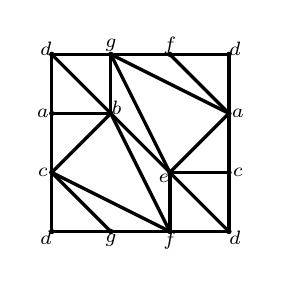
\begin{tikzpicture}[scale = .15]
    \draw[-,very thick] (0,0) -- (15,0) -- (15,15) -- (0,15) -- cycle;
    \draw[-,very thick] (0,5) -- (5,0);
    \draw[-,very thick] (0,5) -- (10,0);
    \draw[-,very thick] (0,5) -- (5,10);
    \draw[-,very thick] (0,10) -- (5,10);
    \draw[-,very thick] (0,15) -- (5,10);
    \draw[-,very thick] (5,10) -- (10,0);
    \draw[-,very thick] (5,10) -- (5,15);
    \draw[-,very thick] (5,10) -- (10,5);
    \draw[-,very thick] (5,15) -- (10,5);
    \draw[-,very thick] (5,15) -- (15,10);
    \draw[-,very thick] (10,0) -- (10,5);
    \draw[-,very thick] (10,5) -- (15,0);
    \draw[-,very thick] (10,5) -- (15,5);
    \draw[-,very thick] (10,5) -- (15,10);
    \draw[-,very thick] (10,15) -- (15,10);
    \filldraw (0,0) circle (5pt);
    \filldraw (5,0) circle (5pt);
    \filldraw (10,0) circle (5pt);
    \filldraw (15,0) circle (5pt);
    \filldraw (15,5) circle (5pt);
    \filldraw (15,10) circle (5pt);
    \filldraw (15,15) circle (5pt);
    \filldraw (10,15) circle (5pt);
    \filldraw (5,15) circle (5pt);
    \filldraw (0,15) circle (5pt);
    \filldraw (0,10) circle (5pt);
    \filldraw (0,5) circle (5pt);
    \filldraw (5,10) circle (5pt);
    \filldraw (10,5) circle (5pt);
    \node at (-.5,-.5) {\scriptsize $d$};
    \node at (5,-.75) {\scriptsize $g$};
    \node at (10,-.75) {\scriptsize $f$};
    \node at (15.5,-.5) {\scriptsize $d$};
    \node at (15.75,5) {\scriptsize $c$};
    \node at (15.75,10) {\scriptsize $a$};
    \node at (15.5,15.5) {\scriptsize $d$};
    \node at (10,15.75) {\scriptsize $f$};
    \node at (5,15.75) {\scriptsize $g$};
    \node at (-.5,15.5) {\scriptsize $d$};
    \node at (-.75,10) {\scriptsize $a$};
    \node at (-.75,5) {\scriptsize $c$};
    \node at (5.5,10.5) {\scriptsize $b$};
    \node at (9.5,4.5) {\scriptsize $e$};
  \end{tikzpicture}
  \end{center}
  \caption{The minimal triangulation of the torus. Image credit: \cite{Lutz}}
  \label{F: torus triangulation}
\end{figure}

The database also contains many triangulations of various interesting
surfaces, such as the torus, Klein bottle, and real projective plane. Below
are the smallest indices (and hence minimal triangulations of) these surfaces
in the database, and see Figure \ref{F: torus triangulation} for a visual
representation of the torus triangulation.

\begin{example}
  \label{E: common surfaces and homology}
\begin{lstlisting}[basicstyle={\ttfamily \scriptsize}, xleftmargin=-23pt]
    i8 : Torus = smallManifold(2, 7, 6, R);
    i9 : KleinBottle = smallManifold(2, 8, 12, R);
    i10 : RP2 = smallManifold(2, 6, 1, R);
\end{lstlisting}
  % 
  We can check that these are the right surfaces by computing their
  homology. Theorems~6.2--6.4 from Munkres confirm that they match
  \cite{Munkres}.
  %
\begin{lstlisting}[basicstyle={\ttfamily \scriptsize}, xleftmargin=-23pt]
    i11 : for i to 2 list prune HH_i Torus
                2    1
    o11 = {0, ZZ , ZZ }
    o11 : List
    i12 : for i to 2 list prune HH_i KleinBottle
    o12 = {0, cokernel | 2 |, 0}
                       | 0 |
    o12 : List
    i13 : for i to 2 list prune HH_i RP2
    o13 = {0, cokernel | 2 |, 0}
    o13 : List
\end{lstlisting}
  % 
  We can explicitly identify the generators of the homology by mapping circles
  onto the torus.
\begin{lstlisting}[basicstyle={\ttfamily \scriptsize}, xleftmargin=-23pt]
    i6 : Circle = skeleton(1, simplexComplex(2,T));
    i7 : f1 = map(Torus,Circle,matrix{{R_3,R_6,R_5}});
    o7 : prints are being ugly
    i8 : prune homology(1, f1)
    o8 = | 1 |
         | 0 |
                  2        1
    o8 : Matrix ZZ  <--- ZZ
    i9 : f2 = map(Torus,Circle,matrix{{R_3,R_0,R_2}});
    o9 : prints are being ugly
    i10 : prune homology(1, f2)
    o10 = | 0 |
          | 1 |
                   2        1
    o10 : Matrix ZZ  <--- ZZ
\end{lstlisting}
  % 
\end{example}

%%%%%%%%%%%%%%%%%%%%%%%%%%%%%%%%%%%%%%%%%%%%%%%%%%%%%%%%%%%%%%%%%%%%%%%%%%%%%%
\subsection{Stanley--Reisner Theory}
\addtocounter{section}{1}
\label{S:Stanley--Reisner Theory}

\noindent
Stanley--Reisner theory connects homological properties of $k[\Delta]$ to
combinatorial and topological properties of $\Delta$. We will discuss some of
the connections here, but a survey of results can be found in
\cites{BH, Stanley, MS}.

Let $\Delta$ be an abstract simplicial complex with vertex set
$V = \{v_0,v_1,\dotsc,v_n\}$, let $k$ be a commutative ring, and let
$S = k[x_0,x_1,\dotsc,x_n]$. The \textbf{Stanley--Reisner ideal} of $\Delta$
is defined to be square-free monomial ideal

$I_\Delta \coloneq \bigl( \prod_{j=1}^k x_{i_j} \mathrel{\big|} \{
v_{i_1},v_{i_2},\dotsc,v_{i_k} \} \not \subset \Delta \bigr) \subset S$
%
\[
  I_\Delta \coloneq \left( \prod_{j=1}^k x_{i_j} \ \bigg\vert \ \{
    v_{i_1},v_{i_2},\dotsc,v_{i_k} \} \not \subset \Delta \right) \subset S,
\]
%
and the \textbf{Stanley--Reisner ring} corresponding to $\Delta$ is
$k[\Delta] = S/I_\Delta$. This correspondence between simplicial complexes and
square-free monomial ideals is one-to-one. Stanley--Reisner theory connects
homological properties of $k[\Delta]$ to combinatorial and topological
properties of $\Delta$. A survey of results can be found in
\cite{BH, Stanley, MS}.

If $I = (m_1, m_2, \dotsc, m_q) \subset S$ is a monomial ideal, with minimal
generators $m_i = \prod x_j^{a_{i_j}}$, then the \textbf{Alexander dual} of
$I$ is defined to be
$I^* \coloneq \bigcap_{i=1}^q (x_0^{a_{i_1}},\ x_1^{a_{i_2}},\dotsc,\
x_{n-1}^{a_{i_{n-1}}})$. If $I = I_\Delta$ for some simplicial complex
$\Delta$, then $I^*$ is also a square-free monomial ideal and is the
Stanley--Reisner ideal of a simplicial complex $\Delta^*$, which we call the
\textbf{Alexander dual} complex to $\Delta$. There is also a combinatorial
description of $\Delta^*$, given by
$\Delta^* = \{ F \subset V \ | \ V \setminus F \not \in \Delta \}$. One of the
attractive features of Alexander duality is the relationship between the
cohomology of $\Delta$ and the homology of $\Delta^*$. More specifically, if
$\Delta$ is a simplicial complex on $n$ vertices, then
$ \widetilde{H}_{i-1}(\Delta^*) = \widetilde{H}^{n-2-i}(\Delta)$ for all
$i \in \mathbb Z$, see \cite[Theorem~5.6]{MS}.
%
% \begin{theorem}[Alexander duality for simplicial complexes]\label{Combinatorial Alexander duality}
%   Let $\Delta$ be a simplicial complex with vertex set $V = \{v_1,v_2,..,v_n \}$. Then
%   %
%   \begin{displaymath}
%     \widetilde{H}_{i-1}(\Delta^*) = \widetilde{H}^{n-2-i}(\Delta)
%   \end{displaymath}
%   %
%   for all $i \in \mathbb Z$.
% \end{theorem}
%
\begin{example}
  \label{Example: Stanley--Reisner ideal and Alexander duality for the bowtie
    complex}
  Consider the simplicial complex $\bowtie$, depicted in
  Figure~\ref{the figure-8 and its dual}.
  %
  \begin{figure}[t]
    \begin{subfigure}{0.3\textwidth}
      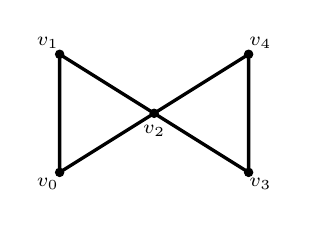
\begin{tikzpicture}[scale = .3]
        % \filldraw[gray!10] (0,0) -- (0,5) -- (4,2.5) -- cycle;
        \draw[-,very thick] (0,0) -- (0,5) -- (4,2.5) -- cycle;
        % \filldraw[gray!10] (8,0) -- (8,5) -- (4,2.5) -- cycle;
        \draw[-,very thick] (8,0) -- (8,5) -- (4,2.5) -- cycle;
        \filldraw (0,0) circle (5pt);
        \filldraw (0,5) circle (5pt);
        \filldraw (4,2.5) circle (5pt);
        \filldraw (8,0) circle (5pt);
        \filldraw (8,5) circle (5pt);
        \node at (-.5,-.5) {\scriptsize $v_0$};
        \node at (-.5,5.5) {\scriptsize $v_1$};
        \node at (4,1.75) {\scriptsize $v_2$};
        \node at (8.5,-.5) {\scriptsize $v_3$};
        \node at (8.5,5.5) {\scriptsize $v_4$};
        % \node at (-2.5,2.5) {\huge $\Delta \hspace{5pt} = $};
      \end{tikzpicture}
%      \caption{The simplicial complex $\Delta$}\label{figure-8 complex}
    \end{subfigure}
    \hspace{50pt}
    \begin{subfigure}{0.3\textwidth}
      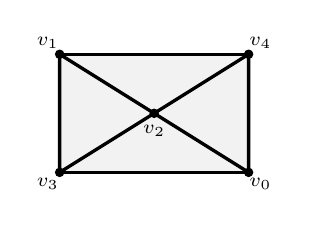
\begin{tikzpicture}[scale = .3]
        \filldraw[gray!10] (0,0) -- (0,5) -- (4,2.5) -- cycle;
        \filldraw[gray!10] (8,0) -- (8,5) -- (4,2.5) -- cycle;
        \filldraw[gray!10] (0,0) -- (8,0) -- (4,2.5) -- cycle;
        \filldraw[gray!10] (0,5) -- (8,5) -- (4,2.5) -- cycle;
        \draw[-,very thick] (0,0) -- (0,5) -- (4,2.5) -- cycle;
        \draw[-,very thick] (8,0) -- (8,5) -- (4,2.5) -- cycle;
        \draw[-,very thick] (0,5) -- (8,5);
        \draw[-,very thick] (0,0) -- (8,0);
        \filldraw (0,0) circle (5pt);
        \filldraw (0,5) circle (5pt);
        \filldraw (4,2.5) circle (5pt);
        \filldraw (8,0) circle (5pt);
        \filldraw (8,5) circle (5pt);
        \node at (-.5,-.5) {\scriptsize $v_3$};
        \node at (-.5,5.5) {\scriptsize $v_1$};
        \node at (4,1.75) {\scriptsize $v_2$};
        \node at (8.5,-.5) {\scriptsize $v_0$};
        \node at (8.5,5.5) {\scriptsize $v_4$};
        % \node at (-2.5,2.5) {\huge $\Delta^* = $};
      \end{tikzpicture}
%      \caption{The Alexandual Dual of $\Delta$}
    \end{subfigure}
    \caption{The simplicial complex $\bowtie$ (left) and its Alexander dual $\bowtie^*$ (right).}\label{the figure-8 and its dual}
  \end{figure}
  The Stanley--Reisner ideal of $\bowtie$ is
  $I_{\bowtie} = (x_0x_1x_2,\ x_0x_3,\ x_1x_3,\ x_0x_4,\ x_1x_4,\
  x_2x_3x_4)$. We can exhibit the correspondence between $\bowtie$ and
  $I_{\bowtie}$ using the methods \texttt{simplicialComplex} and
  \texttt{ideal}.
\begin{lstlisting}[basicstyle={\ttfamily \scriptsize}, xleftmargin=-23pt]
    i28 : S = QQ[x_0..x_4];
    i29 : I$⋈$ = monomialIdeal(x_0*x_1*x_2,x_0*x_3,x_1*x_3,x_0*x_4,x_1*x_4,x_2*x_3*x_4);
    o29 : MonomialIdeal of S
    i30 : $⋈$ = simplicialComplex I$⋈$
    o30 = simplicialComplex | x_3x_4 x_2x_4 x_2x_3 x_1x_2 x_0x_2 x_0x_1 |
    o30 : SimplicialComplex
    i31 : I$⋈$ == ideal $⋈$
    o31 = true
\end{lstlisting}
  We can use the \texttt{dual} method to compute the Alexander dual of
  $\bowtie$.
\begin{lstlisting}[basicstyle={\ttfamily \scriptsize}, xleftmargin=-23pt]
    i133 : dual $⋈$
    o133 = simplicialComplex | x_1x_2x_4 x_0x_2x_4 x_1x_2x_3 x_0x_2x_3 |
    o133 : SimplicialComplex
    i134 : dual(monomialIdeal $⋈$) == monomialIdeal dual $⋈$
    o134 = true
\end{lstlisting}
  % 
  Moreover, we can verify the combinatorial description of $\bowtie^*$ by
  showing that the minimal generators of $I_{\bowtie}$ correspond the
  complements of the facets of $\bowtie^*$.
  % 
\begin{lstlisting}[basicstyle={\ttfamily \scriptsize}, xleftmargin=-23pt]
    i140 : dualFacets = first entries facets dual $⋈$
    o140 = {x x x , x x x , x x x , x x x }
             1 2 4   0 2 4   1 2 3   0 2 3
    o140 : List
    i141 : sort first entries gens I$⋈$ == sort for F in dualFacets list(
               product for v in vertices $⋈$ list(
                   if member(v, support F) then continue else v)
                   )
               )
    o141 = true
\end{lstlisting}
  % 
  Finally, we exhibit the isomorphisms between the cohomology of $\bowtie$ and
  the homology of $\bowtie^*$.
  % 
\begin{lstlisting}[basicstyle={\ttfamily \scriptsize}, xleftmargin=-23pt]
    i94 : all(-1..5, i -> all(-1..5, i -> prune HH^(3-i) $⋈$ == prune HH_(i-1) dual $⋈$)
    o94 = true
\end{lstlisting}  
\end{example}
%
For a simplicial complex $\Delta$ and a face $F \in \Delta$, we define the
\textbf{link} of $F$ to be the subcomplex of $\Delta$ defined by
$\operatorname{link}_\Delta(F) \coloneq \{ G \in \Delta \ | \ F \cup G \in
\Delta \ \text{ and } \ F \cap G = \varnothing \}$. We can now exhibit a more
substantive result of Stanley--Reisner theory, which is the ``dual version''
of Hochster's formula, see \cite[Corollary~1.40]{MS}. This formula allows us
to compute the multigraded Betti numbers of $I_\Delta$, which are defined to
be $\beta_{i,m}(I_\Delta) = \operatorname{Tor}_i^S(I_\Delta, k)_m$. For a
subset $F \subset V$, we will use the notation $\beta_{i,F}$ to refer to the
Betti number in homological degree $i$ and multidegree
$(a_1, a_2, \dotsc, a_n) \in \mathbb{Z}^n$, where $a_i = 1$ if $v_i \in F$ and
$a_i = 0$ otherwise.
%
\begin{theorem}[Hochster's Formula, dual version]
  Let $\Delta$ be a simplicial complex with vertex set
  $V = \{v_0,v_1,\dotsc,v_n\}$ and $S = k[x_0,x_1,\dotsc,x_n]$, where $k$ is a
  field. The nonzero multigraded Betti numbers of $I_\Delta$ and $S/I_\Delta$
  lie in squarefree degrees. Moreover, if $F \subset V$, then
  \[
    \beta_{i,F} (I_\Delta) = \beta_{i+1,F} (S/I_\Delta) = \dim_k \widetilde
    H_{i-1} \big( \operatorname{link}_{\Delta^*}(V \setminus F); k \big) \, .
  \]
\end{theorem}
%
\begin{example}
  In Example \ref{Example: Stanley--Reisner ideal and Alexander duality for
    the bowtie complex}, we computed the Alexander dual of the complex
  $\bowtie$. We can use the \texttt{link} method to compute the links of
  various faces. The link of the central vertex $v_2$ is a square.
  % 
\begin{lstlisting}[basicstyle={\ttfamily \scriptsize}, xleftmargin=-23pt]
    i27 : link(dual $⋈$, x_2)
    o27 = simplicialComplex | x_1x_4 x_0x_4 x_1x_3 x_0x_3 |
    o27 : SimplicialComplex
\end{lstlisting}
  %
  We can also construct a function that computes the multigraded betti numbers $\beta_{i,F}(S/I_{\bowtie})$.
  %
\begin{lstlisting}[basicstyle={\ttfamily \scriptsize}, xleftmargin=-23pt]
    hochster = (i, m) -> (
        G := product select(vertices $⋈$, v -> not member(v, support m));
        rank (homology link(dual $⋈$, G_S))_i
        )
\end{lstlisting}
  %
  Since we have a bound on the nonzero betti numbers of $I_\Delta$, we can collect them into a matrix
  %
\begin{lstlisting}[basicstyle={\ttfamily \scriptsize}, xleftmargin=-23pt]
    i94 : V = vertices $⋈$;
    i95 : squarefreeMonomials = unique sort apply(remove(subsets V, 0), m -> lcm m);
    i96 : matrix for i to length res I$⋈$ - 1 list (
              for F in squarefreeMonomials list hochster(i-1,F)
              )
    o96 = | 0 0 0 0 0 0 0 1 1 0 1 1 0 0 0 1 0 0 0 0 0 0 0 0 1 0 0 0 0 0 0 |
          | 0 0 0 0 0 0 0 0 0 0 0 0 0 0 0 0 1 1 0 0 1 0 0 1 0 1 1 0 1 1 0 |
          | 0 0 0 0 0 0 0 0 0 0 0 0 0 0 0 0 0 0 0 0 0 0 0 0 0 0 0 1 0 0 2 |
                   3        31
    o96 : Matrix ZZ  <--- ZZ
\end{lstlisting}
  %
  where the rows are indexed by the homological degree (starting at $0$), and the columns are indexed by the squarefree multidegrees.
\end{example}
% 
We say that a simplicial complex $\Delta$ is \textbf{pure} if all of the facets of $\Delta$ have the same dimension. We say that $\Delta$ is \textbf{shellable} if we can order the facets $F_1,\dotsc,F_m$ of $\Delta$ so that $\langle F_i \rangle \cap \langle F_1,F_2,\dotsc,F_{i-1} \rangle$ is a pure codimension one simplicial complex. We say that a simplicial complex $\Delta$ is \textbf{Cohen-Macaulay} if $k[\Delta]$ is a Cohen-Macaulay ring. It is known that every shellable simplicial complex is Cohen-Macaulay \cite[Theorem 5.1.13]{BH} and every Cohen-Macaulay simplicial complex is pure \cite[Corollary 5.1.5]{BH}.

% The figure-8 complex from example \ref{Example: Stanley--Reisner ideal and Alexander duality for the bowtie complex} is pure, shellable, and Cohen-Macaulay. Verifying shellability of a simplicial complex can be done using the \texttt{SimplicialDecomposability} package in \texttt{Macaulay2}, \cite{Cook}.

For Stanley--Reisner rings, we can use the combinatorics of $\Delta$ to determine if $k[\Delta]$ is a Cohen-Macaulay ring. Specifically, $k[\Delta]$ is Cohen-Macaulay if and only if $\widetilde H_i(\mathrm{link}_\Delta(F)\; ;\;k) = 0$ for all $F \in \Delta$ and $i < \dim \hspace{2pt} \mathrm{link}_\Delta(F)$, see \cite[Corollary 5.3.9]{BH}. We can also relate the Cohen-Macaulay property to the $h$-vector of $\Delta$. We can write the Hilbert series of $k[\Delta]$ as a rational function
%
\begin{displaymath}
  \sum \dim \hspace{2pt} k[\Delta]_i \hspace{2pt} t^i = \frac {h_0 + h_1t + \cdots h_k t^k}{(1-t)^{d+1}}
\end{displaymath}
%
where $d = \dim \Delta$, and $0 \leq k \leq d+1$ is such that $h_k \not = 0$. If $\Delta$ is a $d$-dimensional Cohen-Macaulay complex with $n$ vertices, then \cite[Lemma 5.1.10]{BH} proves that
%
\begin{displaymath}
  0 \leq h_i \leq \binom{n-d+i}{i}
\end{displaymath}
%
for $i = 0,1,\dotsc,d+1$. We can also compute the $h$-vector using the combinatorics of $\Delta$. Specifically, if $\Delta$ is a $d$-dimensional simplicial complex, then \cite[Lemma 5.1.8]{BH} tells us that
%
\begin{displaymath}
  h_j = \sum_{i=0}^j (-1)^{j-i} \binom{d+1-i}{j-i}f_{i-1}
\end{displaymath}
%
for $j = 0,1,\dotsc,d+1$.
%

%
\begin{figure}[t]
  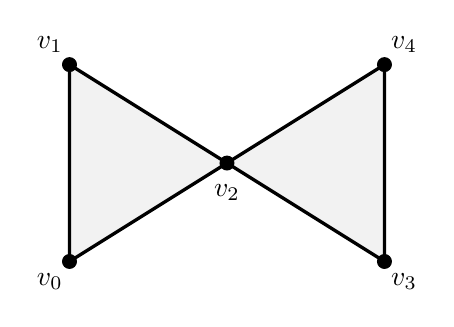
\begin{tikzpicture}[scale = .5]
    \filldraw[gray!10] (0,0) -- (0,5) -- (4,2.5) -- cycle;
    \draw[-,very thick] (0,0) -- (0,5) -- (4,2.5) -- cycle;
    \filldraw[gray!10] (8,0) -- (8,5) -- (4,2.5) -- cycle;
    \draw[-,very thick] (8,0) -- (8,5) -- (4,2.5) -- cycle;
    \filldraw (0,0) circle (5pt);
    \filldraw (0,5) circle (5pt);
    \filldraw (4,2.5) circle (5pt);
    \filldraw (8,0) circle (5pt);
    \filldraw (8,5) circle (5pt);
    \node at (-.5,-.5) {$v_0$};
    \node at (-.5,5.5) {$v_1$};
    \node at (4,1.75) {$v_2$};
    \node at (8.5,-.5) {$v_3$};
    \node at (8.5,5.5) {$v_4$};
    % \node at (-2.5,2.5) {\huge $\Delta \hspace{5pt} = $};
  \end{tikzpicture}
  \caption{The bowtie complex}\label{Figure: the bowtie complex}
\end{figure}
%
\begin{example}
  \label{Example: Shellability, the Cohen-Macaulay property, and the h-vector}
  The simplicial complex $\bowtie$ introduced in example
  \ref{Example: Stanley--Reisner ideal and Alexander duality for the bowtie complex}
  is shellable and Cohen-Macaulay. We can verify the Cohen-Macaulay property
  using \cite[Corollary 5.3.9]{BH}.
  % 
\begin{lstlisting}[basicstyle={\ttfamily \scriptsize}, xleftmargin=-23pt]
    i43 : faceList = flatten for i from -1 to dim $⋈$ list (faces $⋈$)#i
    o43 = {1, x , x , x , x , x , x x , x x , x x , x x , x x , x x }
               0   1   2   3   4   0 1   0 2   1 2   2 3   2 4   3 4
    o43 : List
    i44 : all(faceList, F -> all(0..dim(link($⋈$,F))-1, i -> HH_i link($⋈$,F) == 0))
    o44 = true
\end{lstlisting}
  % 
  However, this package does not provide a method for checking that $\Delta$
  is shellable. Such a method is available in the
  \texttt{SimplicialDecomposability} package in \texttt{Macaulay2}, see
  \cite{Cook}.

  Let us also consider the ``bowtie'' simplicial complex $\fbowtie$, which is
  obtained by filling in the loops of the simplicial complex $\bowtie$, see
  Figure \ref{Figure: the bowtie complex}. Since the intersection of the two
  facets of $\fbowtie$ is a single point, which has codimension two, the
  bowtie complex is not shellable. The simplicial complex $\fbowtie$ is not
  Cohen-Macaulay either, which we can verify by computing the $h$-vector of
  $\fbowtie$.
  %
\begin{lstlisting}[basicstyle={\ttfamily \scriptsize}, xleftmargin=-23pt]
    i3 : I$⧓$ = monomialIdeal(x_0*x_3, x_1*x_3, x_0*x_4, x_1*x_4 );
    o3 : MonomialIdeal of S
    i4 : $⧓$ = simplicialComplex I$⧓$;
    i5 : k$⧓$ = S/I$⧓$;
    i6 : d = dim $⧓$;
    i7 : f$⧓$ = fVector $⧓$
    o7 = {1, 5, 6, 2}
    o7 : List
    i8 : h$⧓$ = for j to d+1 list(
             sum for i to j list (-1)^(j-i)*binomial(d+1-i,j-i)*(f$⧓$#(i))
             )
    o8 = {1, 2, -1, 0}
    o8 : List
\end{lstlisting}
  %
  Since the $h$-vector of $\fbowtie$ has a negative entry, this simplicial
  complex cannot be Cohen-Macaulay, by \cite[Lemma~5.1.10]{BH}.
\end{example}

Some other notable examples of simplicial complexes that are Cohen-Macaulay,
but not shellable, are the Rudin ball and the Ziegler ball. Both of these
complexes are included in the package and can be constructed using the methods
\texttt{rudinBallComplex} and \texttt{zieglerBallComplex} respectively.

%%%%%%%%%%%%%%%%%%%%%%%%%%%%%%%%%%%%%%%%%%%%%%%%%%%%%%%%%%%%%%%%%%%%%%%%%%%%%%
\subsection{Resolutions of Monomial Ideals}
\addtocounter{section}{1}
\label{S:Resolutions of Monomial Ideals}
%

%
Let $\Delta$ be a simplicial complex with $q$ vertices and let
$\widetilde C(\Delta;k)$ be the augmented chain complex of $\Delta$ with
incidence function $\varepsilon$. We will let $S = k[x_0,\dotsc,x_n]$ be a
polynomial ring over the commutative ring $k$, which is typically a field. We
assume that the ring $S$ has the fine $\mathbb N^{n+1}$ grading.

For a monomial ideal $I \subset S$, minimally generated by
$m_1,m_2,\dotsc,m_q$, a \textbf{labelling} of $\Delta$ by $I$ is a bijection
which assigns a minimal generator of $I$ to each vertex of $\Delta$. Without
loss of generality, we will assume this assignment is $v_i \longmapsto m_i$
for $i = 1,2,\dotsc,q$. For each face $F \in \Delta$ we can construct the
monomial $m_F = \mathrm{lcm}(m_i \ | \ i \in F )$. The
$I$-\textbf{homogenization} of $\widetilde{C} (\Delta;k)$ is the chain complex
$(\mathbf G, d)$ such that
%
\begin{displaymath}
  G_0 = S \ \text{ and } \ G_i = \bigoplus_{\dim(F) = i-1}S(m_F).
\end{displaymath}
%
We will use $\{f_F \ | \ F \in \Delta \}$ to denote the canonical basis of $G$ and we define the differential of $\mathbf G$ using
%
\begin{displaymath}
  d(f_F) \hspace{4pt} = \hspace{-8pt} \sum_{\dim(F) = i-1} \frac{m_F}{m_{F'}} \cdot \varepsilon(F,F') f_{F'}.
\end{displaymath}
%
We say that $I$ has a \textbf{resolution supported on} $\Delta$ if the
$I$-homogenization of $\widetilde C(\Delta; k)$ is a free resolution for some
labelling of the vertices of $\Delta$. For further details on
$I$-homogenization, we refer the reader to any one of \cite{BPS, MS, Peeva,
  PV}.
%
\begin{example}
  \label{Example: First example of a homogenized chain complex}
  Let $S = \mathbb Q[x_0,x_1,x_2,x_3]$, let
  $I = (x_0x_1,x_0x_2,x_0x_3,x_1x_2x_3)$, and let $\Gamma$ be the simplicial
  complex with facets $\{ v_1,v_2,v_3 \}$ and $\{ v_2, v_4 \}$.
  % \begin{displaymath}
  %   \begin{tikzpicture}[scale=.35]
  %     \filldraw[gray!15] (0,0) -- (10,0) -- (5,7) -- cycle;
  %     \draw[thick] (0,0) -- (10,0) -- (5,7) -- cycle;
  %     \draw[thick] (5,7) -- (14,6);
  %     \filldraw (0,0) circle (4pt);
  %     \filldraw (10,0) circle (4pt);
  %     \filldraw (5,7) circle (4pt);
  %     \filldraw (14,6) circle (4pt);
  %     \draw node at (-1,0){$v_1$};
  %     \draw node at (11,0){$v_3$};
  %     \draw node at (5,7.7){$v_2$};
  %     \draw node at (15,6){$v_4$};
  %     %     \draw node at (5,-.7){$x_0x_2x_3$};
  %     %     \draw node at (0,4){$\Gamma = $};
  %     %     \draw node at (9.3,3.5){$x_1x_2x_3$};
  %     %     \draw node at (10,7){$x_0x_1x_3$};
  %     %     \draw node at (5,2.5){$x_0x_1x_2x_3$};
  %   \end{tikzpicture}
  % \end{displaymath}
  % 
  If we use the labelling $v_1 \longmapsto x_0x_1$, $v_2 \longmapsto x_0x_2$,
  $v_3 \longmapsto x_0x_3$, and $v_4 \longmapsto x_1x_2x_3$, we get the
  labelled simplicial complex shown in Figure \ref{Figure: Example of a
    labelled simplicial complex}.
  % 
  \begin{figure}[h]\centering
    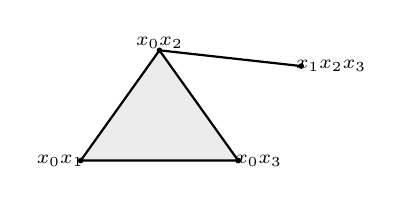
\begin{tikzpicture}[scale=.2]
      \filldraw[gray!15] (0,0) -- (10,0) -- (5,7) -- cycle;
      \draw[thick] (0,0) -- (10,0) -- (5,7) -- cycle;
      \draw[thick] (5,7) -- (14,6);
      \filldraw (0,0) circle (4pt);
      \filldraw (10,0) circle (4pt);
      \filldraw (5,7) circle (4pt);
      \filldraw (14,6) circle (4pt);
      \draw node at (-1.3,0){\scriptsize $x_0x_1$};
      \draw node at (11.3,0){\scriptsize $x_0x_3$};
      \draw node at (5,7.5){\scriptsize $x_0x_2$};
      \draw node at (15.9,6){\scriptsize $x_1x_2x_3$};
      % \draw[blue] node at (5,-.7){\scalebox{.8}{$x_1x_3x_4$}};
      % \draw[blue] node at (0.6,3.5){\scalebox{.8}{$x_1x_2x_4$}};
      % \draw[blue] node at (9.3,3.5){\scalebox{.8}{$x_2x_3x_4$}};
      % \draw[blue] node at (10,7){\scalebox{.8}{$x_1x_2x_4$}};
      % \draw[blue] node at (5,2.5){\scalebox{.8}{$x_1x_2x_3x_4$}};
    \end{tikzpicture}
  \caption{The homogenization of $\Gamma$}\label{Figure: Example of a labelled simplicial complex}
\end{figure}
% 
We can use \texttt{Macaulay2} to compute both $\widetilde C(\Delta; \mathbb Q)$ and the $I$-homogenization of $\Delta$ relative to this labelling, which is the minimal free resolution of $S/I$. 
%
\begin{lstlisting}[basicstyle={\ttfamily \scriptsize}, xleftmargin=-23pt]
    i9 : R = ZZ/101[y_0..y_13];
    i10 : S = QQ[x_0..x_3];
    i11 : $Δ$ = simplicialComplex{R_0*R_1*R_2, R_2*R_3};
    i12 : I = ideal(x_0*x_1,x_0*x_2,x_0*x_3,x_1*x_2*x_3);
    o12 : Ideal of S
    i13 : C = chainComplex $Δ$
            ZZ 1       ZZ 4       ZZ 4       ZZ 1
    o13 = (---)  <-- (---)  <-- (---)  <-- (---)
           101        101        101        101
          -1         0          1          2
    o13 : ChainComplex
    i24 : G = chainComplex($Δ$, Labels => {x_0*x_1,x_0*x_2,x_0*x_3,x_1*x_2*x_3});
    i25 : G.dd
               1                                          4
    o25 = 0 : S  <-------------------------------------- S  : 1
                    | x_0x_1 x_0x_2 x_0x_3 x_1x_2x_3 |
               4                                      4
          1 : S  <---------------------------------- S  : 2
                    {2} | -x_2 -x_3 0    0       |
                    {2} | x_1  0    -x_3 0       |
                    {2} | 0    x_1  x_2  -x_1x_2 |
                    {3} | 0    0    0    x_0     |
               4                    1
          2 : S  <---------------- S  : 3
                    {3} | x_3  |
                    {3} | -x_2 |
                    {3} | x_1  |
                    {4} | 0    |
    o25 : ChainComplexMap
    i15 : (res (S^1/I)) == G
    o15 = true
\end{lstlisting}
%
The $I$-homogenization of $\Delta$ is dependent on how you label the vertices, and that is reflected by the ordering of the monomials in the \texttt{Labels} argument. Indeed, if we swap the labels of $v_1$ and $v_4$, then the $I$-homogenization is no longer a resolution of $S/I$.
%
\begin{lstlisting}[basicstyle={\ttfamily \scriptsize}, xleftmargin=-23pt]
    i22 : G' = chainComplex($Δ$, Labels => {x_1*x_2*x_3,x_0*x_2,x_0*x_3,x_0*x_1});
    i23 : prune homology G'
    o23 = 0 : cokernel | x_0x_3 x_0x_2 x_0x_1 x_1x_2x_3 |
          1 : cokernel {3} | x_3 |                       
          2 : 0                                          
          3 : 0                                          
    o23 : GradedModule
\end{lstlisting}
%
\end{example}
%
Given a monomial ideal $I$, there are several algorithms that will produce a simplicial complex $\Delta$ and a labelling of $\Delta$ by the minimal generators of $I$ such that the $I$-homogenization of $\widetilde C(\Delta; k)$ is a free resolution of $S/I$, though often non-minimally. Examples of such constructions are the Taylor resolution, Lyubeznik resolution, and the Buchberger resolution, all of which are implemented in \texttt{SimplicialComplexes}. We have also implemented a constructor for the Scarf complex, which is a complex that is not always a free resolution of $S/I$, but when it is a free resolution it is minimal. We will not describe these constructions here, but a concise description of the Taylor resolution, Lyubeznik resolution, and Scarf complex is given in \cite{Mermin}, and a description of the Buchberger resolution is given in \cite{OW}. 
% 
\begin{example}
  Consider the monomial ideal $I = (x_1x_3, x_2^2, x_0x_2, x_1^2, x_0^2) \subset \mathbb C[x_0,\dotsc,x_3]$. The Taylor resolution of $I$ can be realized as an $I$-homogenization of the $4$-simplex. 
%  
\begin{lstlisting}[basicstyle={\ttfamily \scriptsize}, xleftmargin=-23pt]
    i2 : R = QQ[a,b,c,d,e];
    i3 : S = QQ[x_0..x_3];
    i4 : I = monomialIdeal(x_1*x_3, x_2^2,  x_0*x_2, x_1^2, x_0^2);
    o4 : MonomialIdeal of S
    i5 : T = taylorResolution J
          1      5      10      10      5      1
    o5 = S  <-- S  <-- S   <-- S   <-- S  <-- S
         0      1      2       3       4      5
    o5 : ChainComplex
    i6 : T == chainComplex(simplexComplex(4,R),Labels => first entries mingens I)
    o6 = true
\end{lstlisting}
  %
  The Buchberger simplicial complex is a subcomplex of the $4$-simplex, and the Buchberger resolution is an $I$-homogenization of the Buchberger simplicial complex. For this example, the Buchberger resolution is the minimal free resolution of $S/I$, but this is not always the case.
  %
\begin{lstlisting}[basicstyle={\ttfamily \scriptsize}, xleftmargin=-23pt]
    i7 : buchbergerSimplicialComplex(J,R)
    o7 = simplicialComplex | acde abcd |
    o7 : SimplicialComplex
    i8 : B = buchbergerResolution J
          1      5      9      7      2
    o8 = S  <-- S  <-- S  <-- S  <-- S
         0      1      2      3      4
    o8 : ChainComplex
    i10 : betti B === betti(res J)
    o10 = true
\end{lstlisting}
  %
Lyubeznik simplicial complexes and resolutions are constructed relative to a total order on the minimal generators of $I$. Every ordering will produce a resolution, but these resolutions need not be isomorphic. When no ordering is given, the methods \texttt{lyubeznikSimplicialComplex} and \texttt{lyubeznikResolution} will order the generators relative to the monomial order on $S$ which, in Macaulay2, is graded revlex by default. The option \texttt{MonomialOrder} reorders the minimal generators of $I$ relative to the monomial ordering on $S$. For example, \texttt{MonomialOrder => \{2,1,0,3,4\}} refers to the total ordering $x_0x_2 <  x_2^2 < x_1x_3 < x_1^2 < x_0^2$ on the minimal generators of $I$. We see that by changing the ordering we can both produce the worst case (Taylor resolution) and best case (minimal free resolution).
  %
\begin{lstlisting}[basicstyle={\ttfamily \scriptsize}, xleftmargin=-23pt]
    i11 : lyubeznikSimplicialComplex(J,R)
    o11 = simplicialComplex | abcde |
    o11 : SimplicialComplex
    i12 : lyubeznikResolution(J) == taylorResolution(J)
    o12 = true
    i13 : lyubeznikSimplicialComplex(J, R, MonomialOrder => {2,1,0,3,4})
    o13 = simplicialComplex | acde abcd |
    o13 : SimplicialComplex
    i14 : L = lyubeznikResolution(J,MonomialOrder => {2,1,0,3,4})
           1      5      9      7      2
    o14 = S  <-- S  <-- S  <-- S  <-- S
          0      1      2      3      4
    o14 : ChainComplex
\end{lstlisting}
  %
The Scarf simplicial complex of $I$ starts with the labelled $4$-simplex and removes any faces $F,F'$ such that $m_F = m_{F'}$. The $I$-homogenization of the Scarf simplicial complex is the Scarf chain complex. It is often the case that the Scarf chain complex is not a free resolution of $S/I$, but when it is a resolution, it is minimal, see \cite[Lemma 3.1]{BPS}.
  %
\begin{lstlisting}[basicstyle={\ttfamily \scriptsize}, xleftmargin=-23pt]
    i16 : scarfSimplicialComplex(J,R)
    o16 = simplicialComplex | acde abcd |
    o16 : SimplicialComplex
    i17 : scarfChainComplex J == buchbergerResolution J
    o17 = true
\end{lstlisting}
\end{example}
%%%%%%%%%%%%%%%%%%%%%%%%%%%%%%%%%%%%%%%%%%%%%%%%%%%%%%%%%%%%%%%%%%%%%%%%%%%%%%
\subsection*{Acknowledgements}
We thank TODO.
               
B.~Hersey was TODO. G.G.~Smith was TODO. A.~Zotine was partially supported by the Natural Sciences and Engineering Research Council of Canada (NSERC).

%%%%%%%%%%%%%%%%%%%%%%%%%%%%%%%%%%%%%%%%%%%%%%%%%%%%%%%%%%%%%%%%%%%%%%%%%%%%%%
\begin{bibdiv}
  \begin{biblist}%[\normalsize]
    
    
    \bib{BH}{book}{
      author={Bruns, Winfried},
      author={Herzog, J\"{u}rgen},
      title={\href{https://doi.org/10.1017/CBO9780511608681}%
        {Cohen-Macaulay rings}},
      series={Cambridge Studies in Advanced Mathematics},
      volume={39},
      publisher={Cambridge University Press, Cambridge},
      date={1993},
      pages={xii+403},
      % isbn={0-521-41068-1},
      % review={\MR{1251956}},
      % doi={10.1017/CBO9780511608681},
    }
    
    \bib{Stanley}{book}{
      author={Stanley, R.P.},
      title={Combinatorics and Commutative Algebra},
      series={Progress in Mathematics},
      volume={41},
      edition={2},
      publisher={Birkh{\"a}user Boston},
      date={1996},
      pages={xi+166}
      % isbn={9780817643690},
    }
    
    \bib{MS}{book}{
      author={Miller, Ezra},
      author={Sturmfels, Bernd},
      title={Combinatorial Commutative Algebra},
      series={Graduate Texts in Mathematics},
      volume={227},
      publisher={Springer-Verlag New York},
      date={2005},
      pages={xiv+420}
      % isbn={9780387237077},
    }
    
    \bib{Peeva}{book}{
      author={Peeva, Irena},
      title={Graded Syzygies},
      series={Algebra and Applications},
      volume={14},
      publisher={Springer-Verlag London},
      date={2011},
      pages={xii+304}
      % isbn={9781447126164},
    }
    
    \bib{Munkres}{book}{,
    author={Munkres, James~R.},
    title={Elements Of Algebraic Topology},
    publisher={CRC Press},
    date={2018},
    pages={x+468}
    % isbn={9780429962462},
    }
    
    \bib{M2}{misc}{
      label={M2},
      author={Grayson, Daniel~R.},
      author={Stillman, Michael~E.},
      title={Macaulay2, a software system for research
        in algebraic geometry},
      publisher={available at \url{http://www.math.uiuc.edu/Macaulay2/}},
    }

    \bib{MFRG}{article}{
      author={\`Alvarez Montaner, Josep},
      author={Fern\'{a}ndez-Ramos, Oscar},
      author={Gimenez, Philippe},
      title={Pruned cellular free resolutions of monomial ideals},
      journal={J. Algebra},
      volume={541},
      date={2020},
      pages={126--145},
      issn={0021-8693},
      review={\MR{4014733}},
      doi={10.1016/j.jalgebra.2019.09.013},
    }

    \bib{BT}{article}{
      author={Bj\"{o}rner, Anders},
      author={Tancer, Martin},
      title={Note: Combinatorial Alexander duality---a short and elementary
        proof},
      journal={Discrete Comput. Geom.},
      volume={42},
      date={2009},
      number={4},
      pages={586--593},
      issn={0179-5376},
      review={\MR{2556456}},
      doi={10.1007/s00454-008-9102-x},
    }
    
    \bib{Cook}{article}{
      author={Cook, David, II},
      title={Simplicial decomposability},
      journal={J. Softw. Algebra Geom.},
      volume={2},
      date={2010},
      pages={20--23},
      issn={1948-7916},
      review={\MR{2881131}},
      doi={10.2140/jsag.2010.2.20},
    }

    \bib{PV}{article}{
      author={Peeva, Irena},
      author={Velasco, Mauricio},
      title={Frames and degenerations of monomial resolutions},
      journal={Trans. Amer. Math. Soc.},
      volume={363},
      date={2011},
      number={4},
      pages={2029--2046},
      issn={0002-9947},
      review={\MR{2746674}},
      doi={10.1090/S0002-9947-2010-04980-3},
    }

    \bib{BPS}{article}{
      author={Bayer, Dave},
      author={Peeva, Irena},
      author={Sturmfels, Bernd},
      title={Monomial resolutions},
      journal={Math. Res. Lett.},
      volume={5},
      date={1998},
      number={1-2},
      pages={31--46},
      issn={1073-2780},
      review={\MR{1618363}},
      doi={10.4310/MRL.1998.v5.n1.a3},
    }

    \bib{Mermin}{article}{
      author={Mermin, Jeff},
      title={Three simplicial resolutions},
      conference={title={Progress in commutative algebra 1},},
      book={publisher={de Gruyter, Berlin},},
      date={2012},
      pages={127--141},
      review={\MR{2932583}},
    }

    \bib{OW}{article}{
      author={Olteanu, Anda},
      author={Welker, Volkmar},
      title={The Buchberger resolution},
      journal={J. Commut. Algebra},
      volume={8},
      date={2016},
      number={4},
      pages={571--587},
      issn={1939-0807},
      review={\MR{3566531}},
      doi={10.1216/JCA-2016-8-4-571},
    }
      
    \bib{Lutz}{article}{
      author={Lutz, Frank H.},
      editor={Bobenko, Alexander I.
      and Sullivan, John M.
      and Schr{\"o}der, Peter
      and Ziegler, G{\"u}nter M.},
      title={Enumeration and Random Realization of Triangulated Surfaces},
      bookTitle={Discrete Differential Geometry},
      year={2008},
      publisher={Birkh{\"a}user Basel},
      address={Basel},
      pages={235--253},
      %isbn={978-3-7643-8621-4},
      %doi={10.1007/978-3-7643-8621-4_12},
    }
    
    \bib{LutzM}{webpage}{
      author={Lutz, Frank~H.},
      title={The Manifold Page},
      url={http://page.math.tu-berlin.de/~lutz/stellar/},
      date={2017},
    }
    
  \end{biblist}
\end{bibdiv}

\raggedright

\end{document}
%%%%%%%%%%%%%%%%%%%%%%%%%%%%%%%%%%%%%%%%%%%%%%%%%%%%%%%%%%%%%%%%%%%%%%
               

%%% Local Variables:
%%% mode: latex
%%% TeX-master: t
%%% End:
$t$